

максимальная высота этого графика отражает степень сжатия в данный момент времени, чем выше уровень сжатия, тем громче звук, это так называемая амплитуда, расстояние между двумя соседними пиками, двумя соседними впадинами или, точнее, длина одного цикла называется длиной волны, чем короче длина волны, тем выше частота звука и, следовательно, тем выше высота звука, который мы слышим \cite{benesty2008microphone}. 

\subsection{Процесс преобразование аналоговый звук в цифровой и обратно}

Теперь рассмотрим, как компьютер сохраняет эту информацию в цифровой аудиофайл, прежде всего важно понимать, что звук — это аналоговое явление, другими словами, его свойства постоянно меняются, поскольку это аналоговая волна, между ними существует бесконечное количество значений громкости, другими словами, громкость варьируется, стоит отметить что частота длина волны зависит обратно пропорционально.

\subsubsection{Процесс преобразование аналоговый звук в цифровой}

Компьютер не может хранить бесконечное количество значений громкости и частоты, поэтому вместо этого звук отбирается через равные промежутки времени, и в каждом интервале записывается числовое значение громкости, в результате получается набор чисел, эти числа являются цифровым представлением исходная волна \cite{salah2021spatial}.

На рисунке (\ref{fig:ampl_and_time}) представлено, цифровое представление исходной волны: 
\begin{figure}[H]
	\centering
	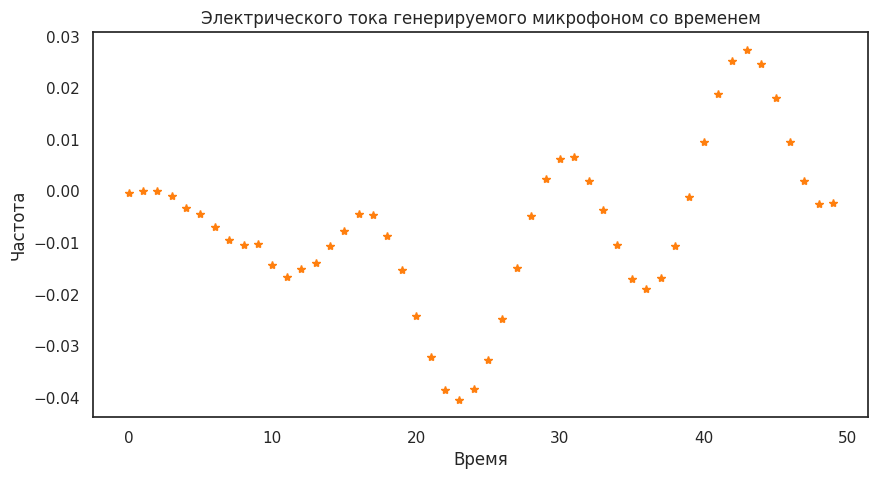
\includegraphics[width=0.8\linewidth]{images/aplitude_and_time.png}
	\caption{Цифровое представление исходной волны}
	\label{fig:ampl_and_time}
\end{figure}

\subsubsection{Процесс преобразование цифровой звук в аналоговый}

Когда цифровая запись воспроизводится, цифровые данные в звуковом файле используются для воссоздания исходной волны. Генерируемый электрический сигнал затем можно усилить и подать на громкоговоритель или наушники, но мы ясно видим, что то, что мы имеем сейчас, является всего лишь приближением. исходного аналогового сигнала это означает, что когда записанный звук воспроизводится, он не совсем такой же, как исходный звук, качество не обязательно такое хорошее, чтобы улучшить качество записи исходной аналоговой волны уменьшают диапазон хранения во временной области, другой стороны это проводит к увлечению размер аудио файла.

На рисунке (\ref{fig:ampl_and_time}) представлено, процесс преобразование цифровой звук в аналоговый: 
\begin{figure}[H]
	\centering
	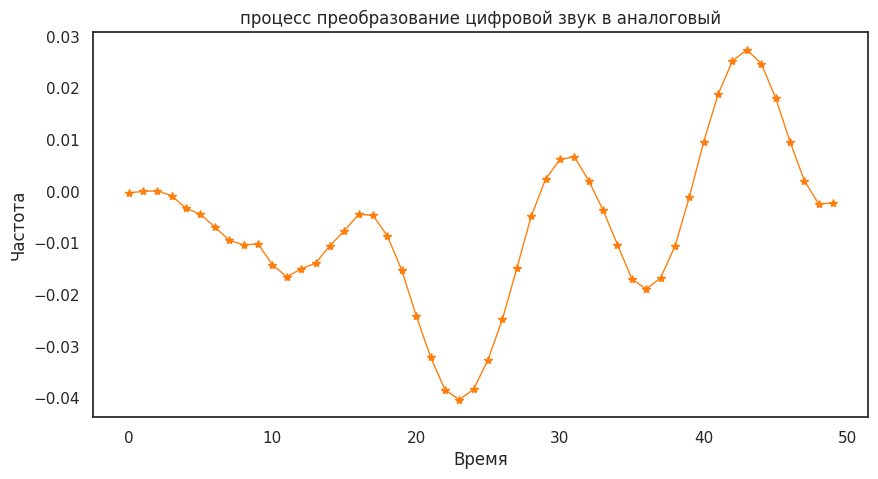
\includegraphics[width=0.8\linewidth]{images/regenration_of_audio.png}
	\caption{процесс преобразование цифровой звук в аналоговый}
	\label{fig:ampl_and_time}
\end{figure}

чтобы уловить высокочастотный звук с любой степенью точности, необходимо дискретизировать волну не менее двух раз за цикл.

Ниже проводим основы характеристики частота дискретизации звука:

\begin{itemize}
    \item выборки в секунду;
    \item измеряется в герцах (Гц);
    \item типичная частота дискретизации составляет 8 кГц для телефонных звонков и передачи голоса через интернет.
\end{itemize}

Важнейшим фактором является количество двоичных цифр, доступных для кодирования громкости каждого образца, так называемая разрядность, предположим на мгновение, что для кодирования значения каждой выборки доступно только три бита, это означает, что каждая выборка может иметь одно из $2^{3} == 8$ возможных значений в диапазоне от нуля до семи, в то время как исходная аналоговая волна дискретизируется, аналого-цифровой преобразователь имеет право чтобы решить, какое из этих восьми значений присвоить каждой выборке в процессе, называемом квантованием, каждое исходное значение должно быть округлено в большую или меньшую сторону до значения, которое можно закодировать, используя только три бита, ошибки округления, возникающие из-за низкой битовой глубины означают, что качество цифровой записи может быть далеко от оригинального звука даже при достаточно высокой частоте дискретизации \cite{liu2023simple}.

\subsection{Форматы хранения аудио в цифровом виде}

Самые популярные аудио форматы на сегодняшний день являются:

\begin{enumerate}
    \item FLAC - наиболее распространенным форматом необработанного несжатого аудио является FLAC, который означает линейную импульсно-кодовую модуляцию, это формат является форматом используемый на аудио компакт-дисках;
    \item WAV - разработано Microsoft и IBM, используется для хранения необработанные аудио-данные;
    \item AIFF - аналог WAV, от Apple для хранения необработанные аудио-данные;
    \item MP3 - один из самых известных форматов сжатого звука, который может уменьшить размер звукового файла до 14 раз.
\end{enumerate}


\section{Синтезированное аудио}

Синтезированное аудио - это недавнее изобретение, которое позволяет пользователям создавать аудиоклипы, которые звучат так, будто конкретные люди говорят то, чего они не говорили. Эта технология изначально разрабатывалась для различных приложений, призванных улучшить жизнь человека, например, для аудиокниг, где ее можно было использовать для имитации успокаивающих голосов \cite{types-of-ad}.


Как определено в литературе по синтезированное аудио, существует три основных типа аудиофейков:

\begin{enumerate}
    \item на основе имитации;
    \item на основе синтеза;
    \item на основе воспроизведения.
\end{enumerate}

\subsection{Аудио дипфейки, на основе имитации}

Данный метод является способом преобразования речи (секретного звука) так, чтобы он звучал как другая речь (целевой звук) с основной целью защиты конфиденциальности секретного звука \cite{detect-fake-imit}.

Голоса можно имитировать разными способами, например, используя людей со схожими голосами, которые могут имитировать исходного говорящего. Однако для имитации звука и речи Deepfake были введены алгоритмы маскировки, такие как Efficient Wavelet Mask (EWM). В частности, исходный и целевой звук будут записаны со схожими характеристиками. 

На рисунке (\ref{fig:imit-deepfake}) представлено, работы система работающий на основе имитации: 
\begin{figure}[H]
	\centering
	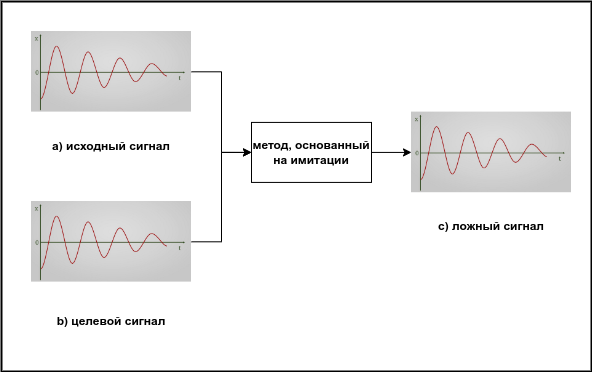
\includegraphics[width=0.5\linewidth]{images/imitation-based-deepfake.png}
	\caption{Система работающий на основе имитации}
	\label{fig:imit-deepfake}
\end{figure}

Судя по рисунке, сигнал исходного звука (\ref{fig:imit-deepfake})(a) будет преобразовано для произнесения речи в целевом аудио на (\ref{fig:imit-deepfake})(b) используя метод генерации имитации, который будет генерировать новую речь (\ref{fig:imit-deepfake})(c), сигнал является ложным и имеет характеристики похоже на целевой сигнал. поэтому людям трудно отличить ложный от реальный звук, созданный этим методом \cite{detect-fake-imit}.

\subsection{Синтетическая основа или преобразование текста в речь}

Синтетическая технология или преобразование текста в речь (TTS) направлена на 
преобразование текста в приемлемый и естественная речь в реальном времени \cite{tan2021survey} и состоит из трёх модулей: 

\begin{enumerate}
    \item модели анализа текста;
    \item акустическая модель;
    \item вокодер.
\end{enumerate}

Чтобы создать синтетический звук дипфейк, необходимо выполнить два важных шага:

\begin{enumerate}
    \item необходимо собрать чистый и структурированный необработанный аудиофайл с расшифровкой аудиоречи;
    \item модель преобразования текста в речь должна быть обучена с использованием собранных данных для построения модели генерации синтетического звука.
\end{enumerate}

В синтетическом методе текст расшифровки с голосом целевого говорящего будет введен в модель генерации, затем модуль анализа текста обрабатывает входящий текст и преобразует его в лингвистические характеристики и затем акустический модуль извлекает параметры целевого говорящего из набора данных в зависимости от лингвистических особенностей, сгенерированных модулем анализа текста. Наконец, вокодер научится создавать речевые сигналы на основе акустических параметров акустических характеристик, и будет сгенерирован окончательный аудиофайл, который включает в себя синтетический искусственный звук в формате волны.

На рисунке (\ref{fig:synth-deepfake}) представлено, синтетический процесс аудио-дипфейк: 
\begin{figure}[H]
	\centering
	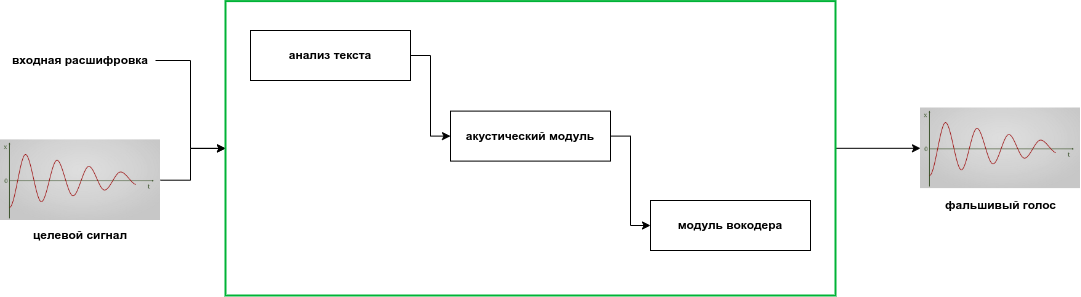
\includegraphics[width=0.8\linewidth]{images/synthetic-based.png}
	\caption{Синтетический процесс аудио-дипфейк}
	\label{fig:synth-deepfake}
\end{figure}

\subsection{Дипфейки на основе повторов}

Дипфейки на основе повторов — это тип вредоносной работы, целью которой является воспроизведение записи голоса целевого говорящего \cite{replay-based-deepfake}, существует два типа дипфейки на основе повторов:

\begin{enumerate}
    \item в дальней зоне;
    \item вырезать и вставить.
\end{enumerate}

При обнаружении в дальней зоне запись жертвы с микрофона воспроизводится как тестовый сегмент на телефонной трубке с громкоговорителем, между тем, вырезание и вставка предполагает подделку предложения, требуемого текстово-зависимой системой \cite{detection-replay-based}.


\section{Связанные темы}

\subsection{Отличительные особенности звука}

Большинство методов используют особую особенность звука для обнаружения его реального или синтетического звука. Целью извлечения признаков является изучение отличительных признаков путем улавливания синтезированных аудио артефактов из речевых сигналов \cite{discrim-features}.
 
\begin{enumerate}
    \item Краткосрочные спектральные особенности;
    \item Долгосрочные спектральные особенности;
    \item Просодические особенности;
    \item Глубокие особенности.
\end{enumerate}



\subsubsection{Мел-частотно-кепстральные коэффициенты (MFCC)}

MFCC отражает закрытую огибающую спектра мощности, которая отражает характеристики речевого тракта и человеческого голоса. Мел-частотный кепстр, сформированный этими коэффициентами, используется для идентификации периодических компонентов сигнала во временной области как пиков в новой области, называемой областью «Частотную» \cite{mfcc-01}. MFCC получаются путем преобразования сигнала из временной области в частотную область, а затем в частотную область из частотной области с использованием ряда математических преобразований \cite{mfcc-02}.

MFCC моделирует спектральное распределение энергии понятным для восприятия способом. Перед расчетом MFCC, чтобы усилить высокочастотные компоненты, следует использовать фильтр верхних частот с конечной импульсной характеристикой (FIR) для предварительного выделения входной речи \(\mathbf{X} = [x(1), x(2), \ldots, x(l), \ldots, x(L)]\) следующим образом:

\begin{equation}
    {x^'}(i) = x(i) - 0.95x(i-1)
\end{equation}

где L — размер входного аудио.

Затем, умножая каждый кадр на окно Хэмминга, сигнал выделения \({x^'}(i)\) разделяется на перекрывающиеся кадры:

\begin{equation}
    \omega(n) = 0.54 - 0.46 \cos(\frac{2 \pi n}{N - 1}), 0 \leq n \leq N - 1,
\end{equation}

где N — длина окна.

Затем частотный спектр получается путем применения быстрого преобразования Фурье (FFT) к каждому оконному кадру. Затем спектр разлагается на несколько под-диапазонов с использованием набора треугольных полосовых фильтров Мел-масштаба.

\begin{equation}
    E(b) = \left\{
    \begin{array}{ll}
    \sum_{k=1}^{N} \text{коэффициент}_k, & \text{если } 0 \leq b \leq B \\
    0, & \text{иначе}
    \end{array}
    \right.
\end{equation}

Теперь MFCC можно рассчитать, применив дискретное косинусное преобразование (DCT) к логарифму \(E(b)\) следующим образом:

\begin{equation}
    MFCC(s) = \sum_{b=0}^{B-1} \log_{10}(1 + E(b)) \cos\left(\frac{s\pi}{B} (b + 0.5)\right), \quad 0 \leq s \leq S
\end{equation}

где S — длина MFCC. 

\subsubsection{кепстральные коэффициенты линейной частоты (LFCC)}

Кепстральные коэффициенты линейной частоты (LFCC) - это метод, аналогичный MFCC, за исключением того, что он использует расположенный набор фильтров на линейной частотной шкале с равномерным разделением между фильтрами, что позволяет получить более высокое разрешение сигнала на высоких частотах \cite{lfcc-00}, поскольку разделение между фильтрами не увеличивается вместе с частотой.

\subsubsection{спектрограм}

Cпектрограммы извлекаются путем разделения звукового сигнала на небольшие перекрывающиеся сегменты и последующего применения преобразования Фурье к каждому из них индивидуально.
Математически это можно определить как:

\begin{equation}
    S_{k,h} = \sum_{n=0}^{N - 1} \omega (n) x(n + hH)e^({-i2\pi n \frac{k}{N})}
\end{equation}

Где \(h = 0, \ldots , T\) – временной интервал, \(k = 0 \ldots \frac{N}{2}\) — частота, \(N\) — количество выборок, которые мы рассматриваем для каждого временного кадра, \(H\) — величина перекрытия, определяемая как размер скачка от одного кадра к другому, а \(\omega(n)\) — оконная функция для уменьшения спектральной утечка из-за нецелого числа периодов гармоник во временном интервале. Поскольку он работает на разных ограниченных сегментов исходных данных, выходная спектрограмма представляет собой комплексную матрицу \(FxT\), где F — количество элементов разрешения по частоте, равное половине размера кадра N для теоремы Найквиста, а T — количество кадров, которые мы анализируем. в форме волны в зависимости от длины сигнала и степени перекрытия.

\subsubsection{Мел-спектрограмма}

Мел-спектрограмма применяет банк фильтров частотной области к аудио-сигналу, который разбит во времени. Мел-Спектрограмма  использует Мел-шкалу для имитации нелинейного частотное восприятие слуховой системы человека, которое является логарифмическим и собирает наиболее важную для восприятия информацию, присутствующую в аудио.

Мел-спектрограмма генерируется путем разделения аудиосигналов на перекрывающиеся кадры с использованием функции оконной обработки. Кратковременное частотное преобразование (STFT) рассчитывается для получения спектрограмм с последующим использованием банков фильтров мел-шкалы для преобразования оси частоты в мел-шкалу, как указано в уравнении: 

\begin{equation}
    m = 2595 * log 10(1 + f / 700) - 1
\end{equation}

где m — масштаб мела, а f — частота в герцах. Наконец, рассчитывается логарифм энергий банка фильтров для получения необходимой мелспектрограммы.

\subsection{Методы для обучения и обнаружения}

\subsubsection{Логистическая регрессия}

Логистическая регрессия - это метод классификации машинного обучения, и его цель состоит в том, чтобы получить модель, которая предсказывает класс выборки и основана на вероятностях \cite{isak2020logistic}. Он используется в задачах бинарной классификации и соответствует данным логистической функции:

\begin{equation}
    h_{\theta}(x) = \frac{1}{1 + e^{-\theta^{T} X}}
\end{equation}

Функция основана на функции сигмойд \cite{fig:sigmoid-func}, представленной в модели с помощью \(\hat{y} = \sigma (\theta^{T})\), которая дает вероятность принадлежности значения к классу, поскольку это задача бинарной классификации, эта функция поможет выбрать между значениями “0” или “1” \cite{javed2012automatic}.

На рисунке (\ref{fig:sigmoid-func}) представлено, график функции сигмойд: 
\begin{figure}[H]
	\centering
	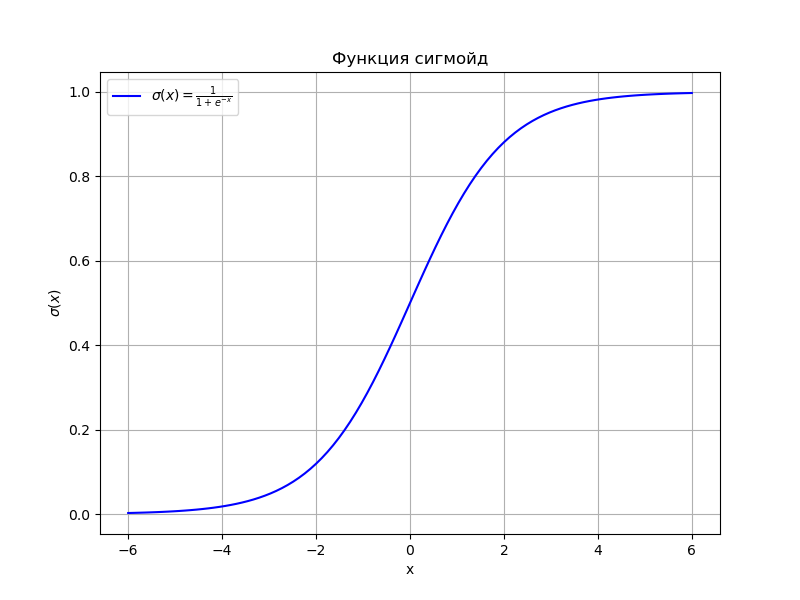
\includegraphics[width=0.8\linewidth]{images/sigmoid.png}
	\caption{Область значение функции сигмойд}
	\label{fig:sigmoid-func}
\end{figure}


Область значение функции зависит от \(\theta^{T} X\), связанная с увеличением функции сигмойд, приближается к единице. с другой стороны, когда \(\theta^{T} X\) уменьшается, функции сигмойд дает значение ближе к нулю. Основная цель состоит в том, чтобы оптимизировать параметр \(\theta\), который обучается. Оптимальные значения параметров находятся, когда функция затрат минимизируется с помощью алгоритма оптимизации. функция затрат выглядит следующим образом:

\begin{equation}
    J(\theta) = - \frac{1}{m} \sum_{i = 1}^{m} [y^{(i)} \log (h_{\theta} (x^{(i)})) + (1 - y^{i}) \log (1 - h_{\theta}(x^{(i)}))]
\end{equation}

Где \(x^{(i)}\) соответствует единичным обучающим данным \(i\), \(y^{i}\) это реальный вывод данных \(i\), \(h\) - прогноз или выходные данные.

Важно проанализировать производительность модели машинного обучения, и для их анализа обычно используются следующие показатели. Матрица ошибок, которая может быть двоичной или многоклассовой. Кроме того, показатели точности, отзыва, оценки F1-мера и общей точности.

Где TP - истинно положительный, FP - ложноположительный, TN - истинно отрицательный, а FN - ложноотрицательный.


На рисунке (\ref{fig:confusion-matrix}) представлено, Матрица ошибок: 
\begin{figure}[H]
	\centering
	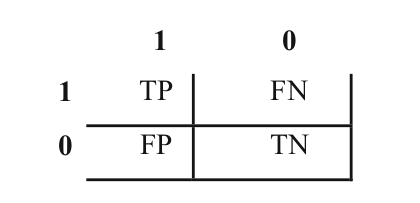
\includegraphics[width=0.8\linewidth]{images/confusion_matrix.png}
	\caption{Матрица ошибок (Confusion matrix)}
	\label{fig:confusion-matrix}
\end{figure}

\textbf{Метрики производительности для классификации:}

\begin{itemize}
    \item Точность (Precision) (P):
    \[
    P = \frac{TP}{TP + FP}
    \]
    
    \item Полнота (Recall) (R) или Чувствительность (Sensitivity):
    \[
    R = \frac{TP}{TP + FN}
    \]
    
    \item F1-мера (F1 Score) (F1):
    \[
    F1 = \frac{2 \times P \times R}{P + R}
    \]
    
    \item Общая точность (Overall Accuracy) (OA):
    \[
    OA = \frac{TP + TN}{TP + FN + FP + TN}
    \]
    
\end{itemize}


Эти показатели полезны при анализе производительности модели, и это зависит от приложения, которое будет иметь модель. Когда разработчик модели хочет выбрать правильные показатели, необходимо проанализировать цели, которые они преследуют, и ожидаемые результаты при валидации и внешнем тестировании. Идеальные результаты имеют погрешность, близкую к нулю, и также необходимо учитывать функцию затрат, которая используется при обучении модели \cite{bengio2017deep}.

% \subsection{Краткосрочные спектральные особенности}

% Кратковременные спектральные характеристики вычисляются в основном путем применения кратковременного преобразования Фурье (STFT) к речевому сигналу \cite{short-term}. Учитывая речевой сигнал \(x(t)\), предполагается, что он квазистационарен в течение короткого периода (например, 25 мс). STFT речевого сигнала \(x(t)\) формулируется следующим образом:

% \begin{math}
%     \centerline{X(t, \omega) = |X(t, \omega)| e^(j\phi(\omega))}
% \end{math} 

% где \(|X(t, \omega)|\) — спектр амплитуды, а \(φ(\omega)\) — фазовый спектр в кадре t и частотном интервале \(\omega\). Спектр мощности определяется как \(|X(t, \omega)|^2\).

% Кратковременные спектральные характеристики в основном состоят из краткосрочных характеристик, основанных на величине и фазе. Обычно немногие характеристики, основанные на величине, выводятся непосредственно из спектра величины, но большинство из них выводятся из спектра мощности. Фазовые характеристики получаются из фазового спектра.

% Характеристики спектра магнитуд напрямую выводятся из спектра магнитуд \cite{short-term}, характеристики спектра мощности получаются из спектра мощности, который, возможно, наиболее хорошо изучен при обнаружении синтезированного звука.

% \subsection{Долгосрочные спектральные особенности}

% Краткосрочные спектральные характеристики не подходят для фиксации временных характеристик траекторий речевых характеристик, поскольку вычисляются покадрово \cite{long-term}. Поэтому были предложены долгосрочные спектральные характеристики для захвата информации на большом расстоянии из речевых сигналов, и исследования показали, что они имеют решающее значение для обнаружения синтезированного звука \cite{long-tem-01}. 
% Долгосрочные характеристики можно грубо классифицировать на четыре типа с точки зрения подходов к частотно временному анализу: 

% \begin{enumerate}
%     \item функции на основе STFT;
%     \item функции на основе преобразование с константой Q (CQT);
%     \item функции на основе преобразования Гильберта (HT);
%     \item функции на основе вейвлет-преобразования (WT).
% \end{enumerate}

% \subsection{Просодические особенности}

% Просодия относится к несегментарной информации речевых сигналов, включая слоговое ударение, интонационные модели, скорость и ритм речи. В отличие от краткосрочных спектральных характеристик с небольшой длительностью, обычно составляющей 20–30 мс, он охватывает более длинные сегменты, такие как звуки, слоги, слова, высказывания и т.д, авторы статьи  \cite{f0} по обнаружению ложного звука в основном учитывали три основные просодические характеристики: F0, продолжительность и энергию. Эти особенности менее чувствительны к канальным эффектам по сравнению со спектральными особенностями  \cite{f0-01}. Они могут предоставлять дополнительную информацию о спектральных характеристиках для повышения эффективности обнаружения синтезированного звука.

% Важные просодические параметры включают основную частоту (F0), продолжительность, распределение энергии, скорость речи и т. д, F0 также известен как шаг. Высота тона синтетической речи отличается от модели естественной речи. Таким образом, синтетическая речь имеет другую среднюю стабильность высоты тона, чем человеческая речь. Кроме того, соартикуляция человеческой речи более плавная и расслабленная, чем у синтетической речи.

% \subsection{Глубокие особенности}

% Вышеупомянутые спектральные особенности и просодические особенности — почти все созданные вручную особенности обладают сильными и желательными репрезентативными способностями. Однако их дизайн имеет недостатки из-за предвзятости из-за ограничений изображений, созданных вручную \cite{deep-0}. Таким образом, глубокие функции призваны заполнить этот пробел. Глубокие функции изучаются с помощью глубоких нейронных сетей, которые можно грубо разделить на: 

% \begin{itemize}
%     \item обучаемые спектральные функции;
%     \item функции контролируемого внедрения;
%     \item функции самоконтролируемого внедрения
% \end{itemize}

\section{Методы обнаружения синтезированного звука (аудио дипфейки)}

Дипфейковый контент появилось не так давно, и соответственно методы которые используетя для создание и генерации таких контентов в основном используют методы машинное или глубокое обучения и соответственно для обнаружения таких контентов тоже используется методы машинное и глубокое обучение.

Усилий многих авторов по разработке решений для обнаружения дипфейковое аудио в целом можно разделить на две основные категории: Первые используют традиционные методы машинного обучения (ML), а вторые подход, основанный на нейронные сети (NN).

\subsection{Методы основанные на машинного обучения}

\subsubsection{Модель с применением логистической регрессии}

Метод в основном делиться на четырех этапах:

\begin{enumerate}
    \item Маркировка данных;
    \item Извлечение характеристика;
    \item Пост-обработка данных;
    \item Применение логистической регрессии.
\end{enumerate}

На этапе маркировки данных, набор данных был создан для того, чтобы обучить модель машинного обучения. После того как аудиозаписи будут записаны, они должно нормализуются. После этого был приведется процесс имитации среди них. в этом моделе аудиозаписи были сгенерируется с использованием метода на основе имитации. Далее присваивается метки “1” для оригинальных аудио-записей и “0” для поддельных.

На этапе извлечение характеристика, Энтропия сигнала использовуется для получения характеристик логистического классификатора. Энтропия рассчитывается по уравнению Шеннона из \cite{shannon1948mathematical} как:

\begin{equation}
    H = - \sum p_{i} \log (p_{i})
\end{equation}

Где \(H\) - энтропия, а \(p_{i}\) - вероятность появления амплитуды \(i\) в звуковом сигнале.

На этапе пост-обработка данных, проводиться эксперимент чтобы определить если характеристики связаны с результатом, значение делаться на двух частей по одному для каждого класса (0 и 1) где 0 для оригинальные и 1 для поддельные аудио с выбранными характеристиками.

На этапе Применение логистической регрессии, Набор данных был разделен на обучающий набор, который составлял \(20\%\) от общего количества примеров, и дегустационный набор \(80\%\) со случайным распределением примеров. Результаты показывают точность \(0,98\), все поддельные аудио-записи были идентифицированы как поддельные аудиозаписи, а несколько оригинальных аудио-записей были классифицированы как поддельные аудиозаписи \cite{rodriguez2020machine}.

\subsubsection{Метод на основе машина квадратичных опорных векторов}

\subsection{Метод на основе GMM}

Данный метод реализован на основе GMM для обнаружения дипфейкового звука  \cite{gmm}. Классификатор, в этом методе состоит из двух моделей гауссовой смеси, которые были обучены индивидуально на реальных и сгенерированных аудио-образцов. Каждая модель состоит из 128 отдельных гауссовских моделей. Распределение Гаусса выбрано здесь в качестве распределения вероятностей для модели смеси, учитывая его уникальные математические свойства и хорошую вычислительную производительность.

\begin{equation}
    \(f(x)\) = \(\log p(x|\theta_r)\) \(-\) \(\log p(x|\theta_g)\)
\end{equation}

где \(\theta_r\) и \(\theta_g\) — параметры Гаусса для реального и сгенерированного распределения звука соответственно, где x — входная функция MFCC.

\subsection{Ванильная рекуррентная нейронная сеть VRNN}

Аудио по своей природе является своего рода последовательными данными, в которых форма сигнала проявляется на разных частотах и амплитудах в разных временных метках \cite{2019-replay}. Ванильная рекуррентная нейронная сеть (RNN) — это простейшая архитектура, предложенная для обработки и обучения на основе последовательных данных. В нашей реализации V-RNN существует скрытое состояние для отслеживания всей исторической информации из предыдущих меток времени. Учитывая ввод в метку времени t, текущее скрытое состояние обновляется скрытым состоянием из последней метки времени и текущим вводом через полностью связанные слои и функция активации. в методе используется скрытое состояние в последней временной метке как представление всего аудио, затем это представление будет передано на два полностью связанных слоя для получения окончательного результата классификации этого аудио-файла.

\begin{equation}
    h_t = \tanh (W^i i_t + W^h h_{t - 1})
\end{equation}

\begin{equation}
    \mathscr{o}_t = W^\mathscr{o}^2 relu(W^\mathscr{o}^1 h_{last})
\end{equation}

где \(W^i\), \(W^h\), \(W^\mathscr{o}^2\), \(W^\mathscr{o}^1\) относится к параметрам входного слоя, скрытого перехода состояний и двух полностью связанных слоев для вывода соответственно.

\subsection{SCNN}

В этом методе используется модель CNN, примененная к представлению Мел-спектрограммы набора аудио-данных, чтобы обеспечить некоторую однородность и стандартизацию с остальными моделями, вместо этого используется функции аудио-сигналов MFCC и LFCC. Характеристика MFCC получается путем логарифмического масштабирования Мел-спектрограммы, в то время как MFCC рассчитывается на основе Мел-спектрограммы в масштабе DB, LFCC аналогичен, но вместо этого получают на основе спектрограммы с линейной фильтрацией в масштабе DB, архитектура модели представлен на рисунке \ref{fig:scnn}:

\begin{figure}[H]
	\centering
	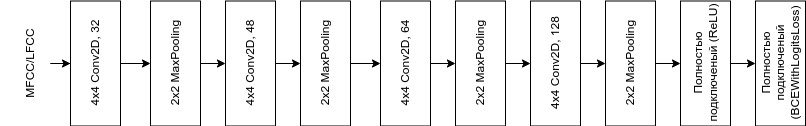
\includegraphics[width=1\linewidth]{images/SCNN.png}
	\caption{Архитектура SCNN}
	\label{fig:scnn}
\end{figure}

Предлагаемая архитектура  SCNN принимает в качестве входных данных двумерное представление аудио-сигнала \(\Bar{X}_\omega\) (MFCC или LFCC) и выводит одно-элементный вектор, указывающий вероятность принадлежности анализируемого аудио к каждому классу (синтез или реальный). Первый и третий сверточные слои состоят из 32 и 64 фильтров размером 4×4 соответственно. Второй сверточный слой состоит из 48 фильтров размером 5×5. Последний сверточный слой состоит из 128 фильтров размером 2 × 4. Все четыре сверточных слоя имеют размер шага 1 × 1 и размер заполнения 1 × 1. последний сверточный слой затем сглаживается и соединяется с полностью связным слоем с помощью функции активации ReLu, выдающей вектор из 128 элементов. Последний полностью связный слой выводит одно-элементный вектор, используемый для получения окончательного результата двоичной классификации, т. е. человека или бота. Метка 0 будет означать, что аудио-сигнал классифицируется как поддельный (синтезированный), а метка 1 будет означать, что аудио-сигнал классифицируется как настоящий (реальным человеком).

Диапазон и область функции активации, которая используется в этой архитектуре нейронной сети:
\begin{equation}
    ReLU(x) = \begin{cases}
    x, & \text{если } x > 0 \\
    0, & \text{иначе}
\end{cases}
\end{equation}


\subsection{TSSD}

Метод использует глубокие нейронные сети (DNN) для извлечения признаков, а также классификации, нейронная сеть принимает необработанные аудио-сигналы без каких-либо предварительных преобразований или вычислений вручную \cite{svdnn}, архитектура нейронные сети представлено на рисунке \ref{fig:tssd}.

\begin{figure}[H]
	\centering
	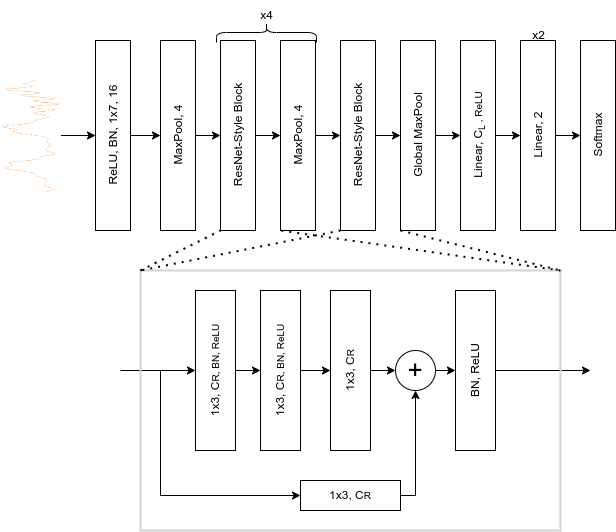
\includegraphics[width=0.7\linewidth]{images/TSSD.png}
	\caption{Архитектура TSSD}
	\label{fig:tssd}
\end{figure}

Первый блок представляет собой одномерный сверточный слой 1x7 с 16 каналами, за которым следует пакетная нормализация (BN), активация ReLU и MaxPool с размером ядра 4. Далее модули в стиле ResNet \cite{last-one} складываются 4 раза со слоем MaxPool размера ядра 4.
Каждый из этих модулей имеет 3 слоя свертки размером 1x3, выходные данные которых объединяются с исходным входом, преобразованным сверткой 1x1 с применением BN и ReLU в конце каждого из этих слоев.

Наконец, за этим следуют 3 полностью связанных слоя (где \(C_{L}\), выходная размерность, равна 128 для первого линейного слоя, 64 для второго и 32 для последнего), а выходные данные создаются слоем softmax, где будет проверяться конечный результат, является ли аудио файл синтезированным или реальным.


% Для классификации реальных и поддельных аудио записей авторы выделили два подхода:
% \begin{enumerate}
%     \item На основе признаков с использованием алгоритмов машинного обучения;
%     \item На основе изображений с использованием алгоритмов глубокого обучения.
% \end{enumerate}

% В подходе классификации на основе признаков аудио-файл преобразуется в набор данных на основе признаков, состоящий из различных спектральных характеристик образцы, эти характеристики далее вводятся в алгоритмы машинного обучения, чтобы различать аудио образцы как настоящие или поддельные \cite{division-of-file}.

%  В подходе классификации на основе изображений аудио-файл переводится на образцов в виде спектрограмм или мел-спектрограмм, которые в дальнейшем подаются в качестве входных данных в алгоритмы глубокого обучения, которые определяют, является ли данный экземпляр аудио реальным или поддельным \cite{division-of-file}.

% \subsection{Метод на основе SVM}

% На рисунке (\ref{fig:synth-deepfake}) представлено, признакы MFCC и схема работы алгоритма классификации SVM: 
% \begin{figure}[H]
% 	\centering
% 	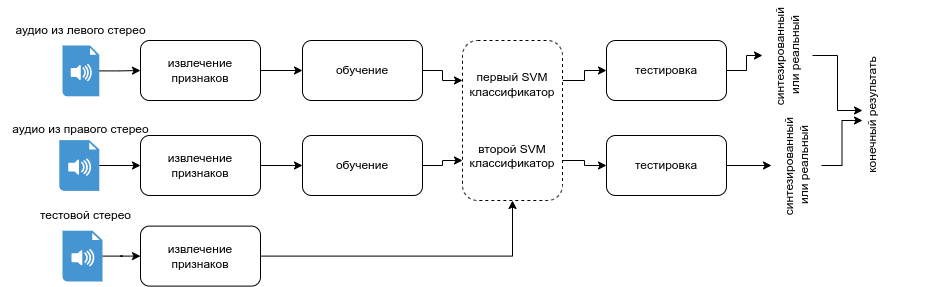
\includegraphics[width=0.8\linewidth]{images/svm.png}
% 	\caption{Признакы MFCC и схема работы алгоритма классификации SVM}
% 	\label{fig:efficient-cnn}
% \end{figure}

% \subsection{EfficientCNN}

% Слово Efficient в переводе с англ, переводиться как эффективный и CNN как сверточная нейронная сеть этот отдел нейронные сети часто применяется для изучения и исследование над изображениями, входными данными для модели EfficientCNN является нормализованная мел-спектрограмма, который обрабатывается посредством блокировки обработки ввода и четырех блоков свертки, выходные данные слоя объединения после последнего блока свертки передаются в блок классификации для получения прогнозов классификатора \cite{efficient-cnn}.

% На рисунке (\ref{fig:synth-deepfake}) представлено, архитектура модель EfficientCNN: 
% \begin{figure}[H]
% 	\centering
% 	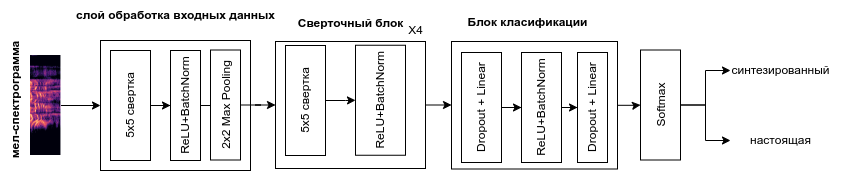
\includegraphics[width=0.8\linewidth]{images/efficient-cnn.png}
% 	\caption{Модель, состоящая из блока входной обработки, 4 блоков свертки и блока классификации}
% 	\label{fig:efficient-cnn}
% \end{figure}

% Теперь опишем каждый из этих блоков подробно:

% \begin{itemize}
%     \item \textbf{блок обработка входных данных} - Блок обработки ввода принимает нормализованную входную мел-спектрограмму и пропускает ее через 2d-слой свертки с ядром 5x5, слой активации ReLU, слой пакетной нормализации и слой максимального пула.
%     \item  \textbf{Блок свертки} - Каждый блок свертки состоит из свертки 1x1, ReLU, пакетной нормализации, свертки 3x3, еще одного ReLU и еще одной пакетной нормализации, выходные данные этого блока проходят через слой максимального пула 2x2, прежде чем стать входными данными для другого сверточного или
%     классификационный блок.
%     \item \textbf{Блок класификации} - Блок классификации состоит из линейного слоя, ReLU, слоя пакетной нормализации и еще одного линейного слоя с отсевом, включенным перед каждым линейным слоем. Выходные данные окончательного линейного слоя передаются на слой softmax для создания прогнозов модели.
% \end{itemize}

